\section{序論}
執筆要領について述べる。

\subsection{用紙}
A4用紙を縦長に使用する。本文は8ページ(表裏で4枚)以上、24ページ以内を標準とする。

\subsection{ヘッダ・フッタ}
ヘッダの左側には、「筑波大学大学院博士課程システム情報工学研究科修士論文」につづけて、修了年度・月を括弧書きで記述する。
ヘッダの右側には、氏名を記述する。氏名については、見やすくするために適宜空白をいれても差し支えない。

フッタの中央には、ページ番号をハイフンはさんで記述する。

\subsection{1ページ目の体裁}
申請する学位(修士(工学))を四角囲みで記述し、
つづけて修士論文のタイトルをそれぞれ日英表記で記述する。
ただし本文が英文の場合、英日の順に記述する。

つぎに、氏名・所属専攻と指導教員名・指導教員の所属を日英表記で記述する。
氏名・指導教員名については、見やすくするために適宜空白をいれても差し支えない。
ただし本文が英文の場合、英日の順に記述する。


\subsection{要約・キーワード}
修士論文の概要を記述する。
本文が日本語・英語に係らず概要は英語で記述する。


\subsection{本文}
本文は2段組みとし、10.5pで記述する。
句読点は、各分野で用いられる記号を使用する。

\subsection{図表}
論文として印刷に耐えうる品質(解像度)の図表を作成する。
図表中、および、キャプションは、原則として英語を使用する。
キャプションは、図の下と表の上に挿入する。
図番号および表番号は、それぞれ Figure 1、Table 1 のように表記する。
横長の図・表の場合は、段抜きで挿入してもよい。

たとえば、Figure \ref{fig:samplefigure}や Table \ref{tbl:sampletable}を例として示す。

\begin{figure}[t]
    \centering
    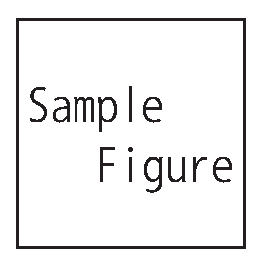
\includegraphics{sample.eps}
    \caption{Sample figure}\label{fig:samplefigure}
\end{figure}

\begin{table}
    \centering
        \caption{Sample table} \label{tbl:sampletable}
        \begin{tabular}{c|ccc}
            A & B & C & D\\
            \hline \hline
            a & b & c & d\\
            a & b & c & d\\ \hline
        \end{tabular}
\end{table}

\subsection{数式}
数式のサンプルとして、(\ref{eq:gauss})を示す。
\begin{equation}
 \int _\infty ^\infty e^{-x^2}dx = \sqrt{\pi} \label{eq:gauss}
\end{equation}

\subsection{参考文献}
それぞれの分野の記述法により、十分な数の参考文献を引用する\cite{Kanai2000BED}。著者が執筆した修士論文に関連する内容の論文等がある場合には、必ず文献として引用する。

\subsection{著者紹介}
学会誌論文の一般的な著者紹介を例に記述する。

\subsection{付録}
本文には書ききれないデータなどは、
付録に収めることができる。付録は、研究室で別途保管する。



\section{\LaTeX スタイルファイルについて}
このサンプルは、筑波大学大学院システム情報工学研究科知能機能システム専攻の修士論文を\LaTeX で作成するためのスタイルファイルである。
配布ファイルは以下の通りである。
\begin{description}
 \item[iit-jp-sjis.sty]  知能機能システム専攻の修士論文のためのスタイルファイル
 \item[templete.tex] スタイルファイルを利用するためのテンプレートファイル
 \item[face.eps] 顔写真用のテスト画像
 \item[sample.eps] Figure のためのテスト画像
\end{description}

スタイルファイルやテンプレートは、適宜改良をして使用してもよい。

\section*{謝辞}
本研究は、・・・・・・深謝する。


\vspace{2\jsZw}
\noindent
\begin{minipage}{\columnwidth}
    \begin{wrapfigure}[6]{l}[-4pt]{30mm} 
        \centering
        
\includegraphics[width=30mm]{face.eps}
    \end{wrapfigure}
    \noindent 筑 \ 波 \ 太 \  郎\\\\
    筑波大学大学院システム情報工学研究科知能機能システム専攻所属
\end{minipage}

\vspace{6\jsZw}
\noindent----------------------------------------------\par

\begin{itemize}
 \item Webで公開する論文の概要は、別に作成する。
 \item 修士論文は両面印刷とする。
 \item 修士論文提出時は、ソフトカバーを施して必要部数を大学院教務に提出する。背表紙は不要。
 \item 論文審査後に、両面印刷したもの(綴じていないもの)を専攻長に提出する。
 \item 専攻長は、専攻全員の修士論文をハードカバーにて製本し、専攻室で保管する。
\end{itemize}

\begin{itemize}
 \item Extended summary is also required for uploading onto the web.
 \item The thesis should be printed in double face printing.
 \item Submit your thesis to the academic service office. The thesis should be clapped with a soft-cover.
 \item  Submit your thesis to the chair of the iit, after it has passed the examining meeting. The thesis should not be clapped.
 \item The chair of the iit will bind up all the accepted theses and preserve in his/her office.
\end{itemize}